%% ---------------------------------------------------------------
%% Supplementary Information
%% Reset counters and prefix figures/equations/tables with "S"
%% ---------------------------------------------------------------
\setcounter{equation}{0}
\setcounter{figure}{0}
\setcounter{table}{0}
\setcounter{section}{0}
\renewcommand{\theequation}{S\arabic{equation}}
\renewcommand{\thefigure}{S\arabic{figure}}
\renewcommand{\thetable}{S\arabic{table}}

%% ---------------------------------------------------------------

\subsection*{S1.\; KMS functional connectivity and equilibrium interpretation}

The Kubo-Martin-Schwinger (KMS) formalism provides a rigorous characterization of
thermal equilibrium in systems with infinitely many degrees of
freedom~\cite{haag1967quantum}. A system is in thermal equilibrium at temperature $T$
when its correlation functions between observables satisfy an analytic condition relating
forward and time-reversed observables via a shift in complex time determined by the
inverse temperature $\beta = 1/(k_B T)$.

Recent work extends the KMS formalism to directed networks by modeling information flow
using graph algebras~\cite{raeburn2005graph, moutuou2025kubo, moutuou2025brain}. In this
setting $\beta$ acts as a propagation scale parameter controlling the relative
contribution of paths of different lengths: large $\beta$ emphasizes short, direct paths,
whereas smaller $\beta$ allows longer and recurrent pathways to contribute. This provides
a principled link between equilibrium statistical physics and probabilistic information
flow on networks.

\subsection*{S2.\; Graph algebra formulation and neural emittance}

The \emph{C.~elegans} connectome is modeled as a directed network $G=(V,E)$ comprising
302 neurons and 16,857 directed edges obtained by combining the chemical synapses and gap
junctions provided in the datasets by Varshney~\emph{et al.} and Cook~\emph{et
al.}~\cite{varshney2011structural, cook2019connectome}. Let $\mathbf{A}$ denote the
adjacency matrix.

The KMS construction assigns to each neuron $v$ a state $\mathbf{x}^{v|\beta}$,
representing the distribution of signals originating from $v$ under equilibrium
propagation. For target neuron $u$, the value of $\mathbf{x}^{v|\beta}$ is given by
\begin{equation}
\mathbf{x}^{v|\beta}_{u}
=
\frac{1}{Z^{\beta}_{v}}
\left(
\sum_{\mu:\,v\to u} e^{-\beta |\mu|}
\right),
\label{eq:SI_emittance}
\end{equation}
where the sum is over all directed walks $\mu$ of any length from $v$ to $u$, $|\mu|$ is
the number of synapses traversed, and $Z^{\beta}_{v}$ is a partition function quantifying
the total communication capacity of $v$ at inverse temperature $\beta$. Because the graph
contains cycles and self-loops, this series converges only for $\beta > \beta_c$, where
\begin{equation}
e^{-\beta_{c}} = \frac{1}{r(\mathbf{A})}, \qquad \beta_{c} = \log r(\mathbf{A}),
\end{equation}
with $r(\mathbf{A})$ the spectral radius of $\mathbf{A}$. In this regime the emittance
admits the resolvent form
\begin{equation}
\mathbf{x}^{v|\beta}_{u} = \frac{1}{Z^{\beta}_{v}}
\left( \mathbf{I} - e^{-\beta}\,\mathbf{A} \right)^{-1}_{uv},
\end{equation}
which captures both direct and higher-order pathways, integrating local and global
contributions to functional connectivity.

\subsection*{S3.\; Mixed KMS states and entropy}

Network-level equilibrium patterns are obtained by mixing neuron-specific KMS states
\begin{equation}
\mathbf{x} = \sum_{v} p_v \, \mathbf{x}^{v|\beta},
\end{equation}
where $\{p_v\}$ is a probability distribution over neurons. To quantify the dispersion of
information flow we compute the Shannon entropy of the resulting distribution. Higher
entropy indicates more distributed communication, whereas lower entropy reflects
concentration along a smaller set of pathways.

\subsection*{S4.\; Selection of functional inverse temperature}

Entropy was evaluated across a range of $\beta$ using multiple neuron-weighting schemes
(in-degree, out-degree, total degree, and standard reference distributions). We selected
$\beta = 5.103$, which maximizes entropy across all weighting schemes while remaining
within the convergence regime (Fig.~\ref{fig:SI_entropy}), corresponding to a maximally
distributed yet stable communication regime.

\subsection*{S5.\; Dataset description}

The synaptic connectome was assembled by merging two datasets: the physical connectome of
\emph{C.~elegans} reported by Varshney~\emph{et al.}~\cite{varshney2011structural} and
the whole-animal connectomes of both sexes published by Cook~\emph{et
al.}~\cite{cook2019connectome}. All edges from both datasets were combined to produce a
comprehensive connectome containing 302 neurons and 16,857 directed edges, which served
as input for the KMS functional connectivity computation. The neuropeptidergic connectome
published by Ripoll-S\'{a}nchez~\emph{et al.}~\cite{ripoll2023neuropeptidergic} was used
as the extrasynaptic layer for comparison.

\subsection*{S6.\; Null model and statistical significance}

To assess the dependence of functional interactions on synaptic topology, we generated
5,000 degree-preserving randomized networks. Each null network preserves the in-degree
and out-degree of every neuron while randomizing edge
placement~\cite{fosdick2016configuring}. For each neuron pair, the observed KMS emittance
value was compared to the null distribution; edges exceeding the 95th percentile ($p <
0.05$) were classified as significant, isolating interactions specifically constrained by
network topology rather than degree alone.

\subsection*{S7.\; Subgraph classification and network analysis}

Functional subgraphs were defined by intersecting KMS-derived edges with the extrasynaptic
connectome:
\begin{itemize}
  \item \textbf{Topology-dependent extrasynaptic} --- extrasynaptic edges overlapping
        with significant KMS edges.
  \item \textbf{Topology-resilient extrasynaptic} --- extrasynaptic edges overlapping
        with non-significant KMS edges.
  \item \textbf{Purely extrasynaptic} --- extrasynaptic edges absent from KMS
        connectivity entirely.
  \item \textbf{Purely synaptic} --- significant KMS edges without extrasynaptic
        support.
\end{itemize}

These subgraphs define functional communication regimes rather than intrinsic neuron
classes. For each subgraph, network statistics including degree, weighted degree, and
neuron-type composition were computed. Motor neurons dominated the topology-dependent
network, interneurons were prominent in the topology-resilient network, survival-critical
neurons (CAN, M4, I1) were concentrated in the purely extrasynaptic subgraph, and sensory
neurons were most strongly represented in the purely synaptic subgraph, consistent with
its role in rapid reflexive behavior.

\subsection*{S8.\; Topology-dependent regime: reinforcement of synaptic motor circuits}

This regime is enriched for locomotion-related neurons, including DB05, DA07, VA10, and
AS08 (motor; locomotion) and PVDL/R (sensory;
mechanosensation)~\cite{wormatlas2023,chatzigeorgiou2010specific}. High-degree nodes show
in-degree dominance, consistent with convergence of signaling onto motor hubs. Other
nodes, such as VB07, AVBL, and AVBR (motor; locomotion), exhibit higher out-degree,
indicating broadcast roles within locomotor circuits~\cite{wormatlas2023,zhen2015}. This
directional organization, together with the close structural correspondence to the SIFC,
indicates that these extrasynaptic pathways reinforce synaptic motor communication and may
enhance circuit robustness under perturbation (Fig.~\ref{fig:SI_cde}).

\subsection*{S9.\; Topology-resilient regime: global modulation decoupled from synaptic
wiring}

This regime is dominated by interneurons such as AVK (AVKL/AVKR; 232 in- and out-edges
each for AVKL) and PVQ, known for coordination roles, together with RIM, RIB, and DVA,
which occupy central cross-layer positions bridging the synaptic and extrasynaptic
layers~\cite{wormatlas2023,ji2023proprioceptive,marquina2024antagonism,wadsworth1996neuroglia,
bentley2016multilayer}. URX (sensory; oxygen sensing) is also prominent, linking
environmental signals to distributed network
responses~\cite{wormatlas2023,cheung2005experience,gray2004oxygen,zimmer2009neurons}.
Connectivity is typically balanced between in- and out-degree. In contrast, pharyngeal
neurons (e.g., M3, I2R) are absent, confirming that this regime is organized around a
broad synaptic--extrasynaptic interface rather than local
microcircuits~\cite{wormatlas2023,dent1997avr}. The persistence of this structure under
degree-preserving randomization indicates a stable modulatory layer with weak dependence
on precise wiring (Fig.~\ref{fig:SI_cie}).

\subsection*{S10.\; Purely extrasynaptic regime: survival and homeostasis beyond synaptic
reach}

This regime is enriched for neurons linked to survival and homeostasis, including CANL
(457 connections), M1 (449), I1L/R, CANR (402), and M4 (196). I1 and M1 regulate feeding
by coupling sensory input to pharyngeal
output~\cite{wormatlas2023,trojanowski2014neural,bhatla2015light}, while M4 is required
for peristalsis and effective food transport~\cite{wormatlas2023,trojanowski2014neural,
song2012serotonin}. These neurons are sparsely connected in the synaptic connectome but
highly connected extrasynaptically; key members (CANL/R, M4) are individually required
for organismal viability~\cite{chien2019enigmatic}. This contrast indicates that critical
physiological functions in this regime rely predominantly on extrasynaptic communication,
which acts as a primary --- not merely modulatory --- signaling substrate
(Fig.~\ref{fig:SI_peg}).

\subsection*{S11.\; Purely synaptic regime: fast sensorimotor processing without
extrasynaptic support}

This regime captures significant KMS-derived interactions without extrasynaptic support
(2,649 significant vs.\ 28,301 non-significant connections). It is enriched for
sensorimotor neurons: RME (motor; head movement), PHC (sensory; environmental sensing),
AS (motor; locomotion coordination), and FLP (sensory;
mechanosensation)~\cite{kaplan1993,wormatlas2023,bhattacharya2019plasticity,altun2009high,
wang2024neurotransmitter,pereira2015cellular,tolstenkov2018functionally}. RMEL/RMER and
PHCL/PHCR are major hubs by total degree, although many of their connections are
non-significant, indicating that high degree does not necessarily reflect
topology-specific enrichment. By contrast, AS10 and FLPL concentrate the largest number
of significant connections. Overall, this regime supports fast, low-latency sensorimotor
communication where direct synaptic transmission is essential (Fig.~\ref{fig:SI_psg}).

%% ---------------------------------------------------------------
\subsection*{Supplementary Figures}
%% ---------------------------------------------------------------

\begin{figure*}[htbp]
\centering
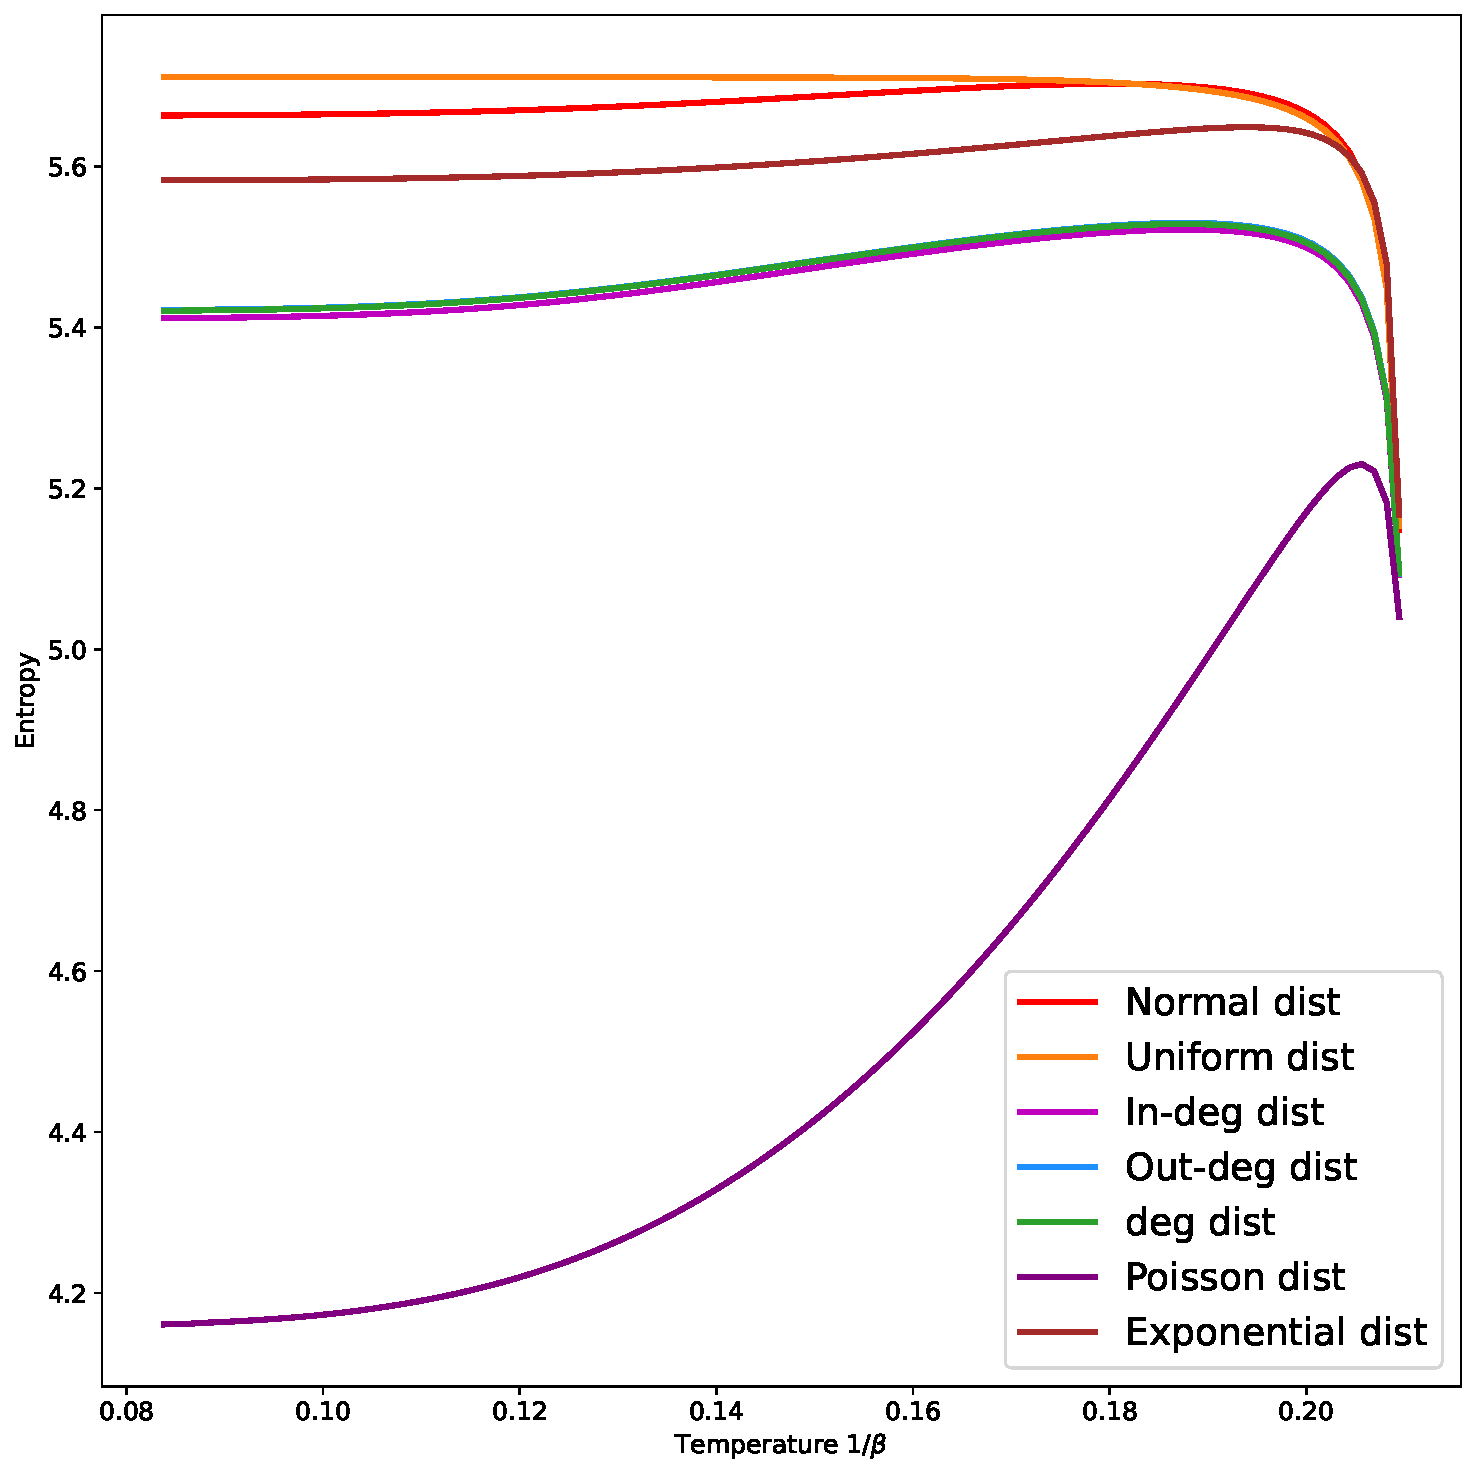
\includegraphics[width=0.6\textwidth]{./SI-figs/entropy.pdf}
\caption{\textbf{Entropy of the mixed emittance distribution as a function of inverse
temperature.} Shannon entropy of the mixed KMS state as a function of $1/\beta$ for
seven neuron-weighting schemes (in-degree, out-degree, total degree, normal, uniform,
Poisson, and exponential distributions). The selected value $\beta = 5.103$ maximizes
entropy across all weighting conditions while remaining within the convergence regime,
corresponding to maximally distributed yet stable information flow.}
\label{fig:SI_entropy}
\end{figure*}

\begin{figure*}[htbp]
\centering
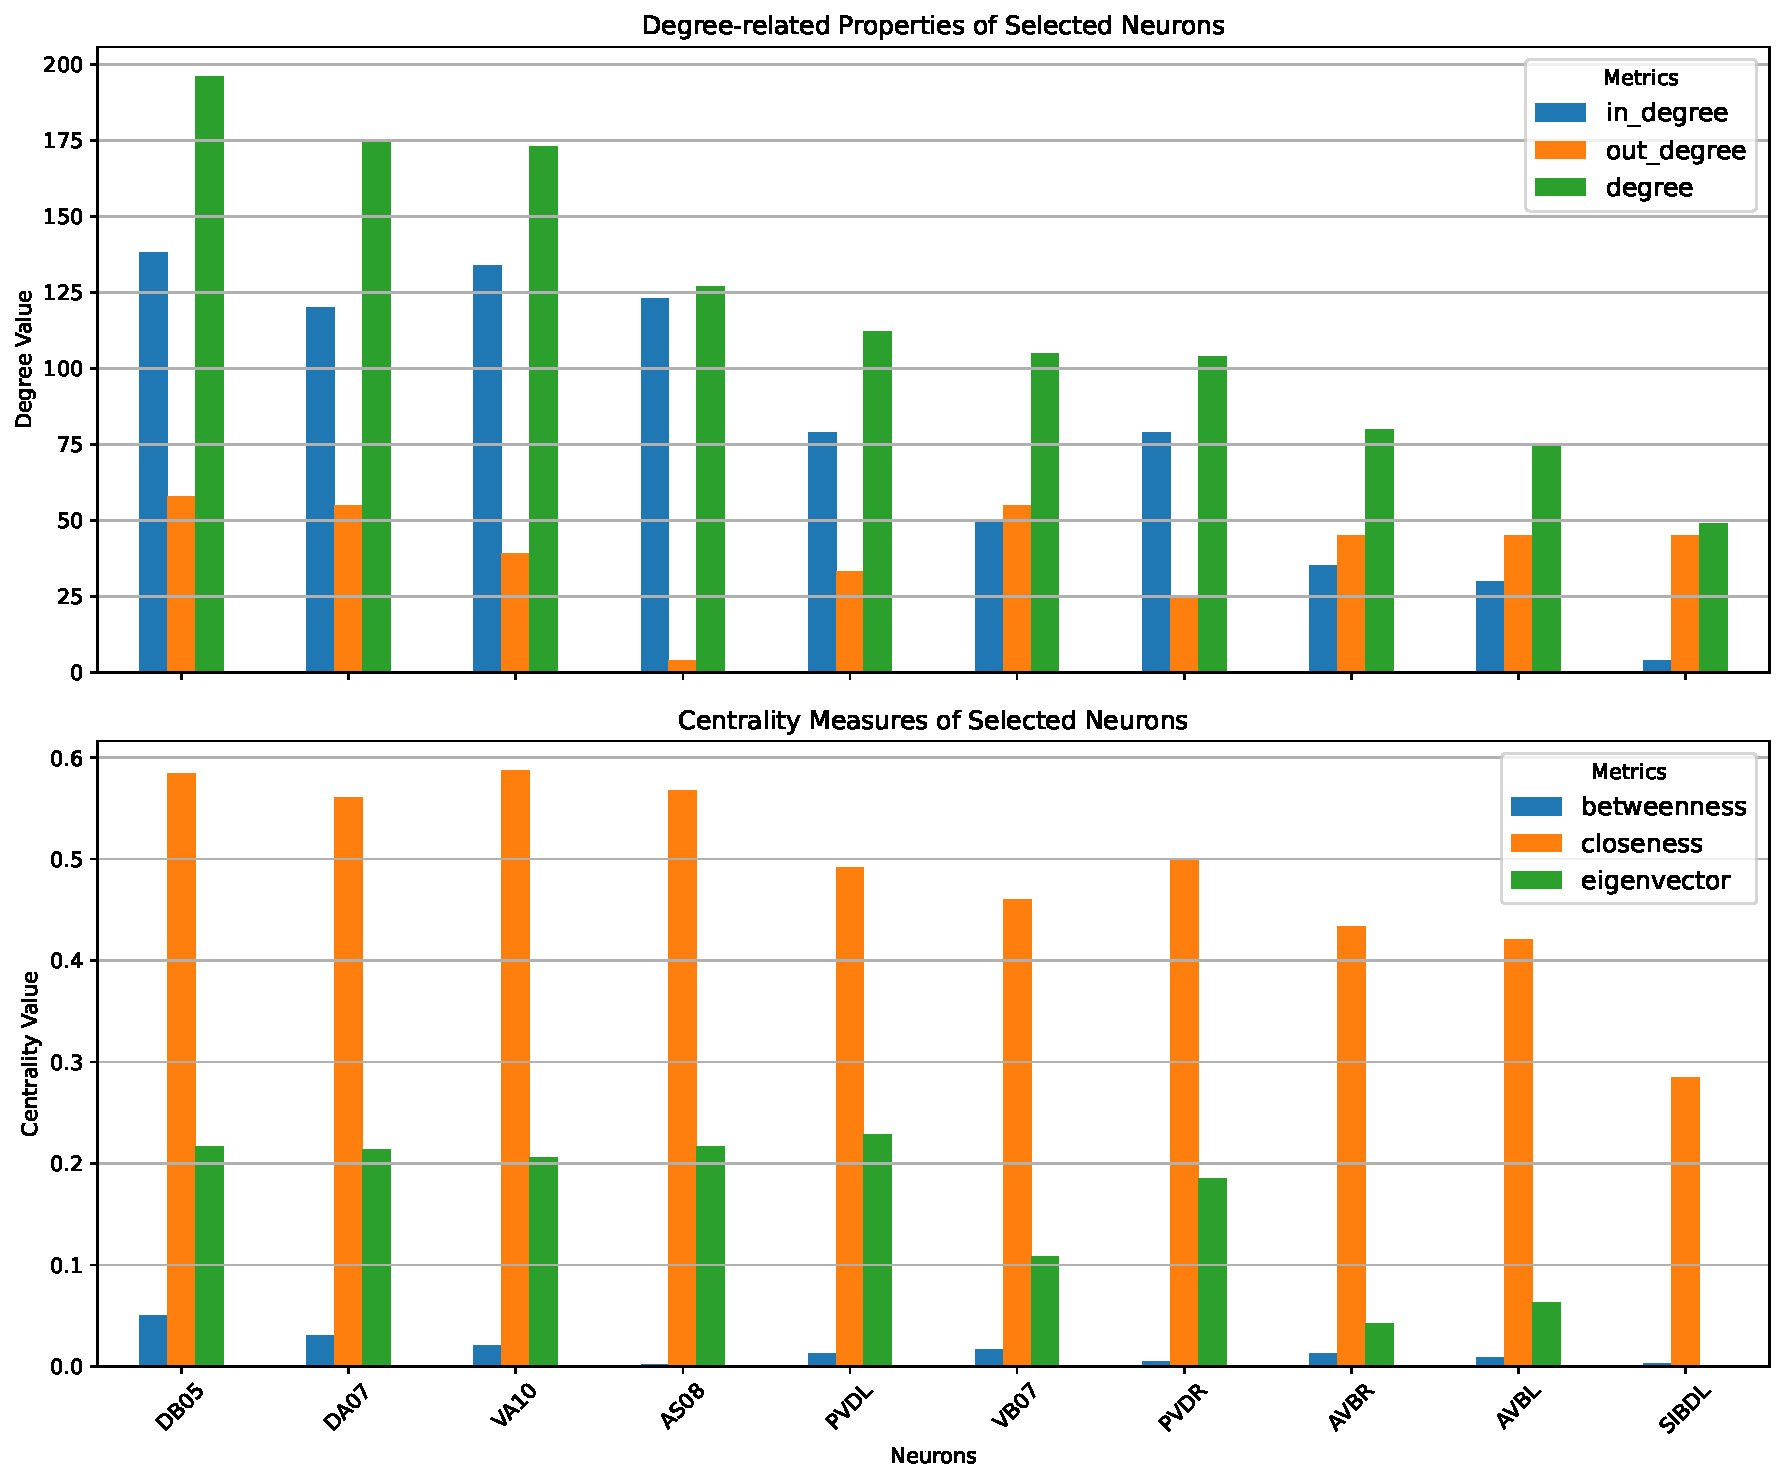
\includegraphics[width=0.6\textwidth]{./SI-figs/cde.pdf}
\caption{\textbf{Connectivity and centrality measures for the topology-dependent
extrasynaptic subgraph.} Degree (in, out, total) and centrality measures (betweenness,
closeness, eigenvector) for the highest-degree neurons within this regime. In-degree
dominance is visible for key locomotion motor neurons (DB05, DA07, VA10, AS08), consistent
with convergence of signaling onto motor hubs, while VB07, AVBL, and AVBR show higher
out-degree reflecting broadcast roles.}
\label{fig:SI_cde}
\end{figure*}

\begin{figure*}[htbp]
\centering
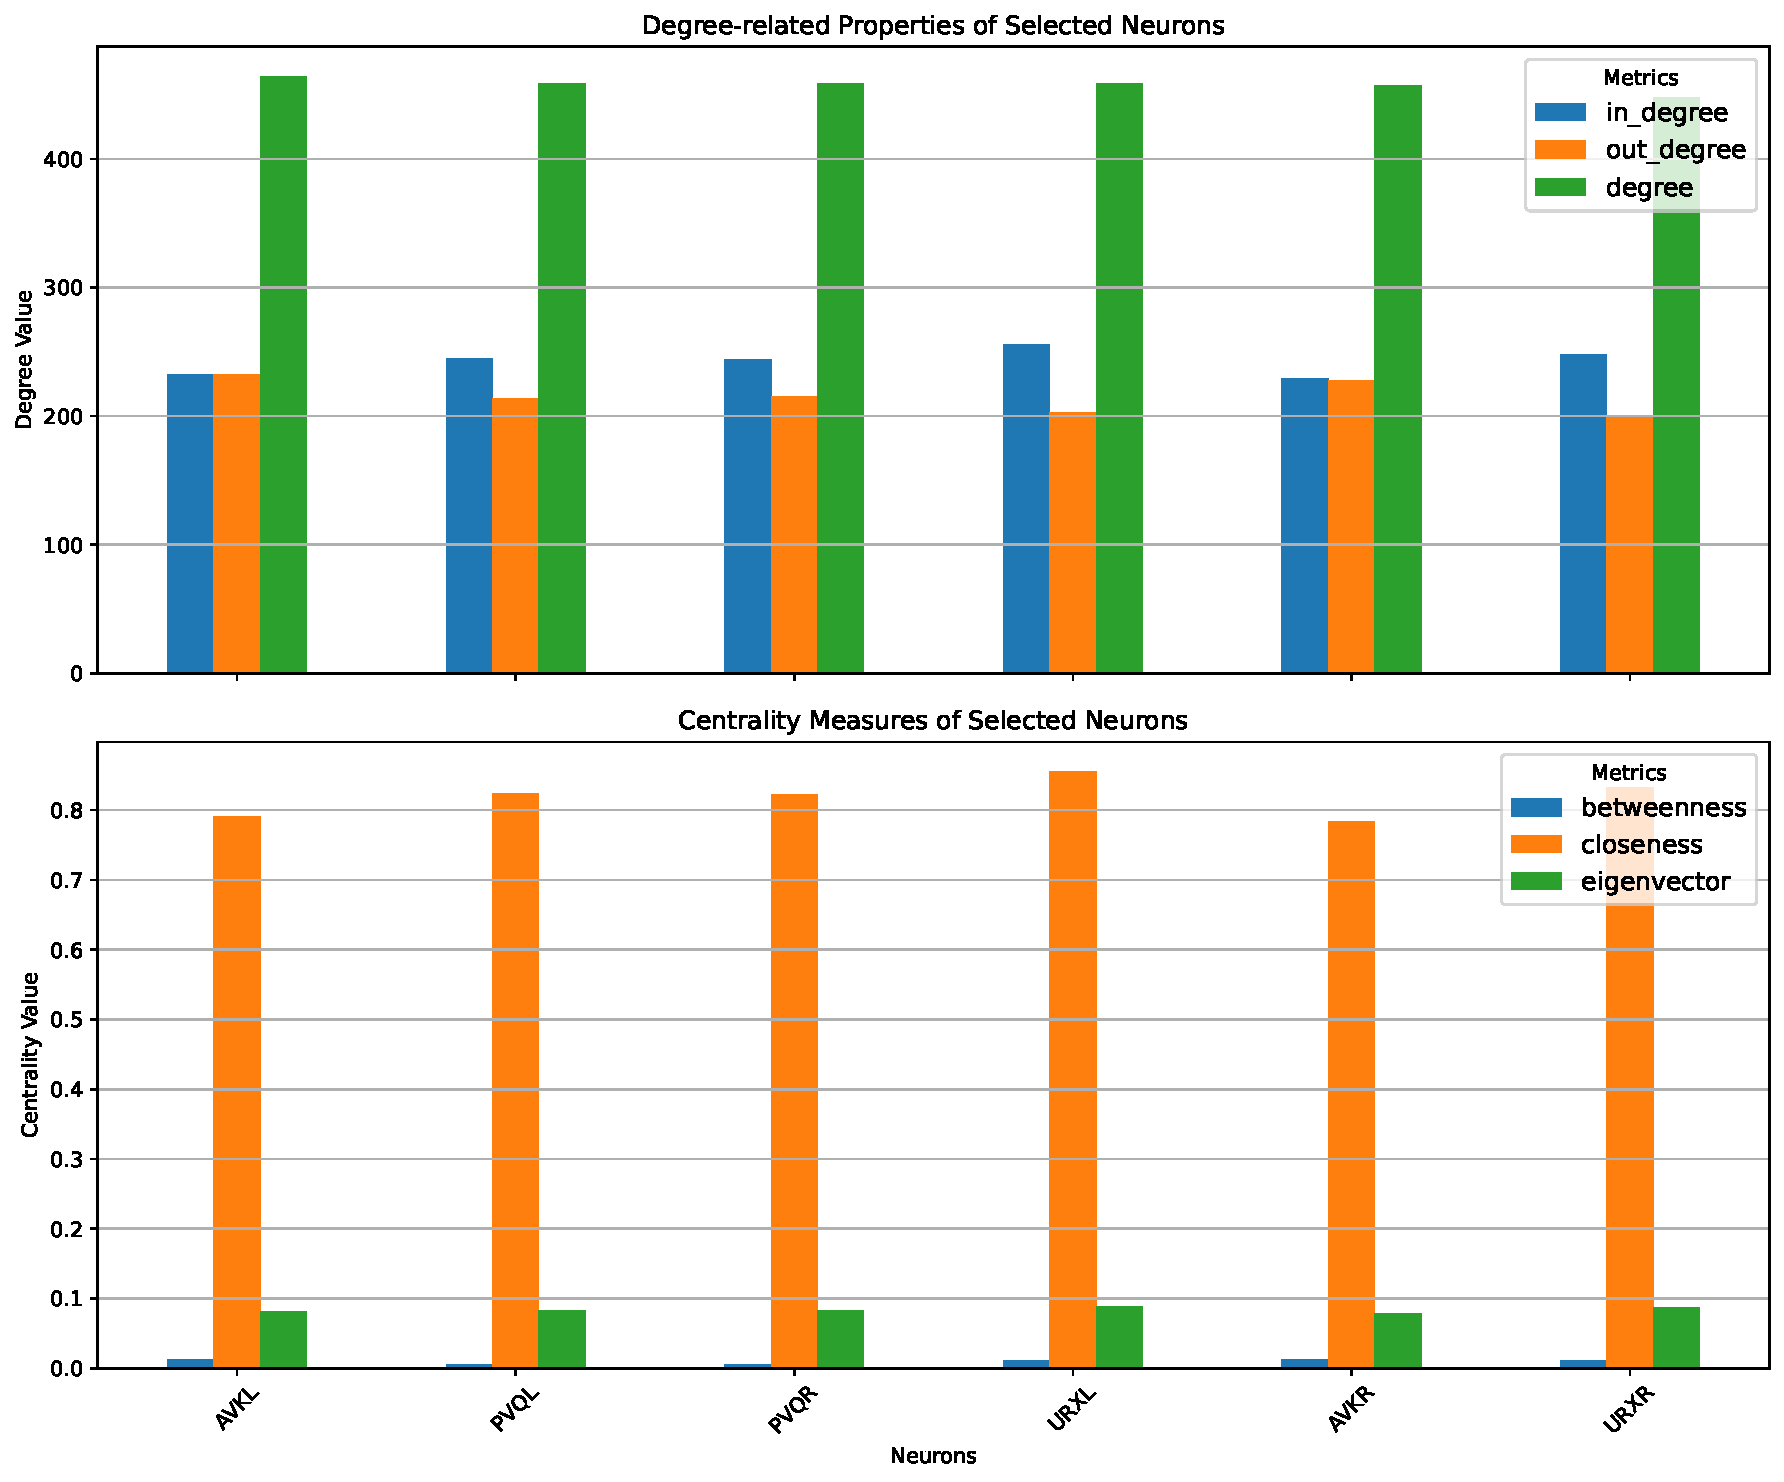
\includegraphics[width=0.6\textwidth]{./SI-figs/cie.pdf}
\caption{\textbf{Connectivity and centrality measures for the topology-resilient
extrasynaptic subgraph.} Degree and centrality measures for representative highly
connected neurons in this regime. Balanced in- and out-degree is characteristic across
nodes, reflecting the distributed modulatory role of this layer. AVKL/AVKR, PVQL/PVQR,
and URXL/URXR form a symmetric, highly connected core.}
\label{fig:SI_cie}
\end{figure*}

\begin{figure*}[htbp]
\centering
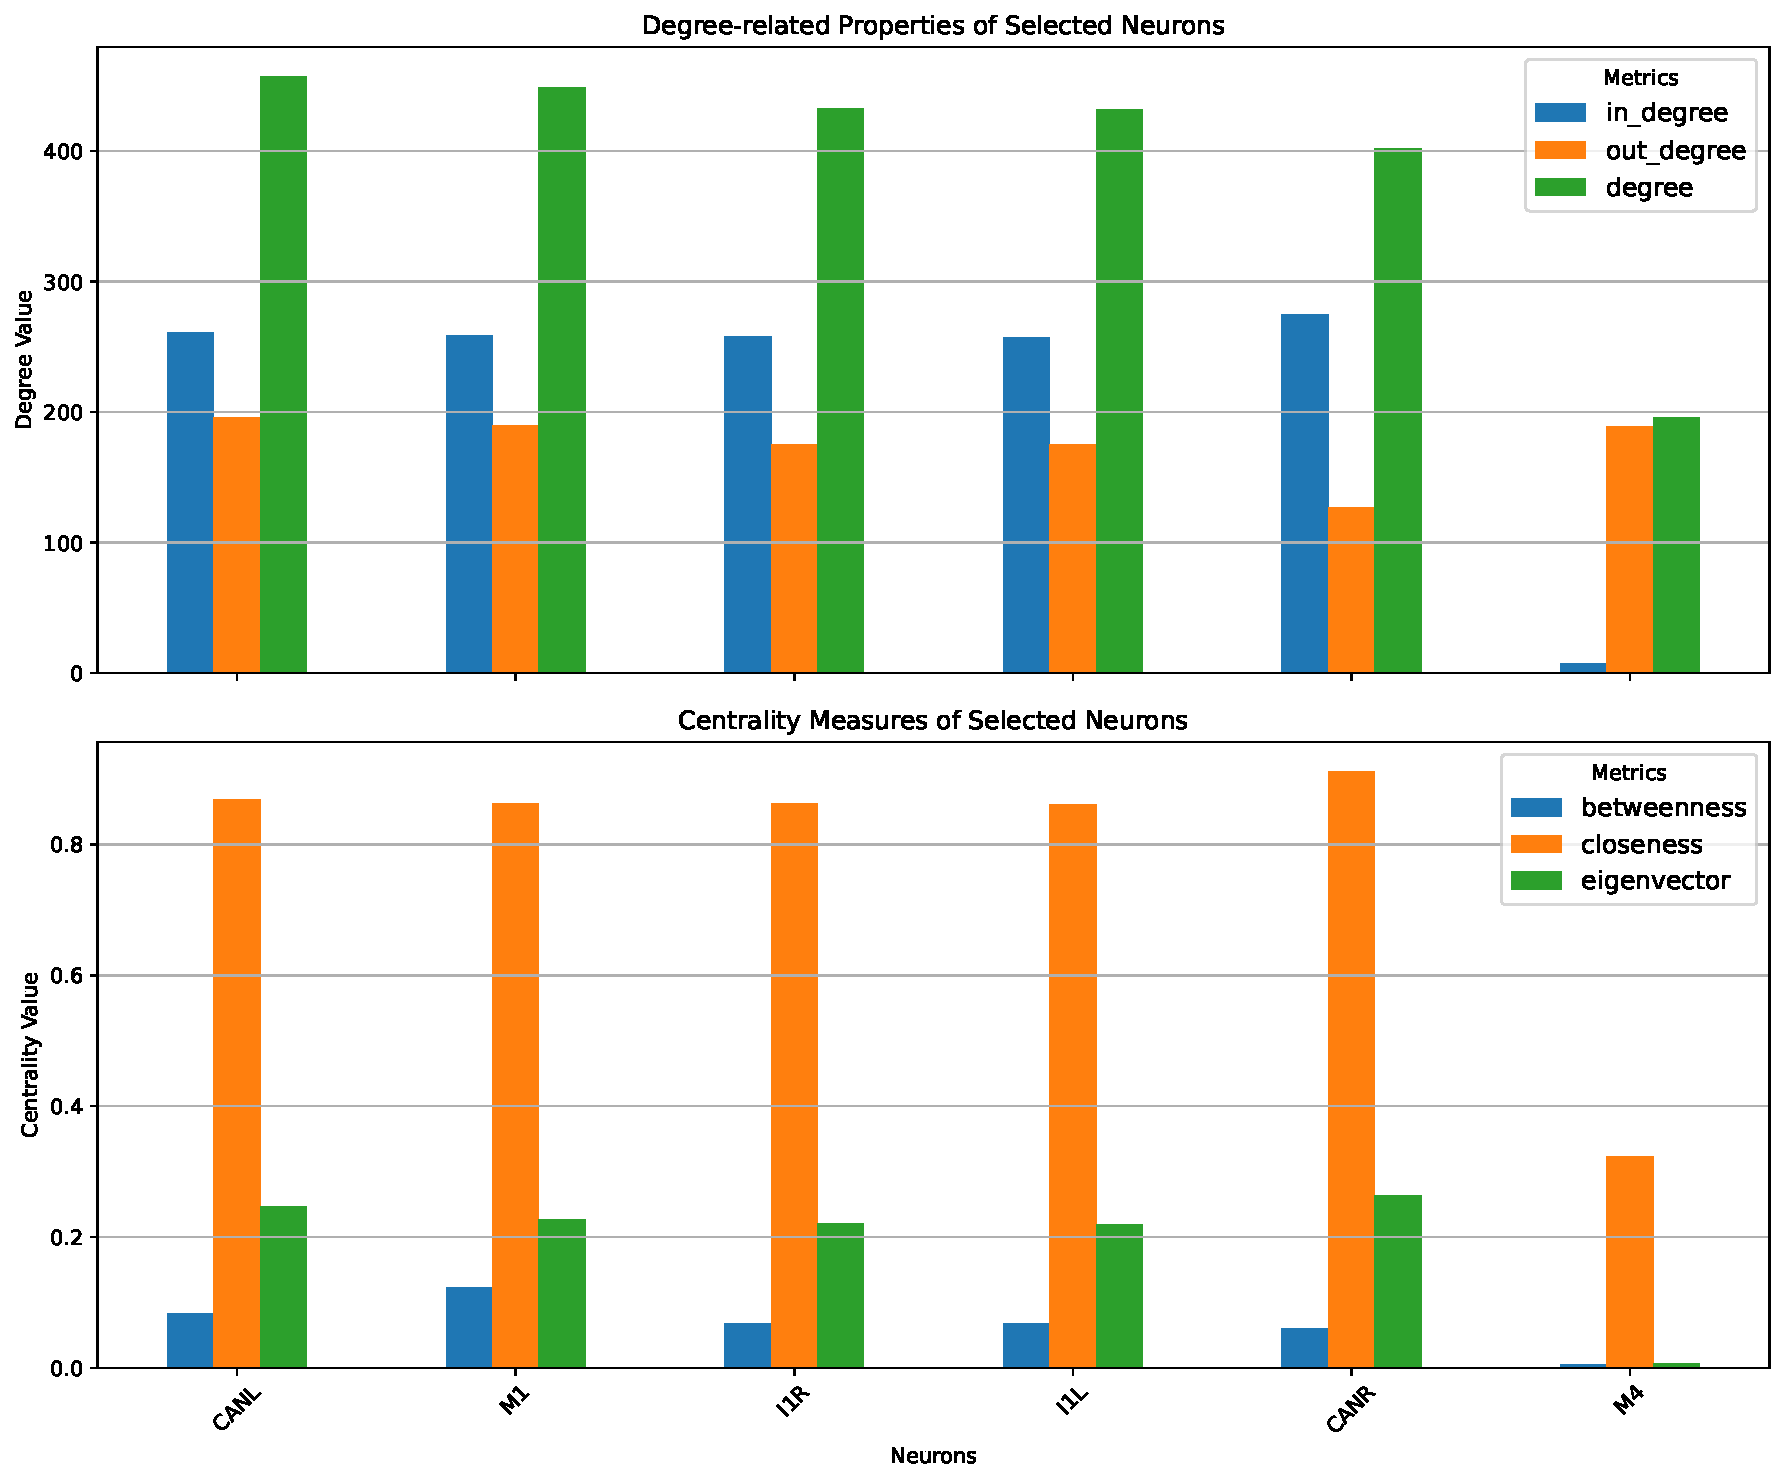
\includegraphics[width=0.6\textwidth]{./SI-figs/peg.pdf}
\caption{\textbf{Connectivity and centrality measures for the purely extrasynaptic
subgraph.} Degree and centrality measures for the most connected neurons within this
regime, including CANL, M1, I1R, I1L, CANR, and M4. These neurons are sparsely connected
in the synaptic connectome but highly connected extrasynaptically, highlighting their
reliance on diffusive signaling for survival-critical and homeostatic functions.}
\label{fig:SI_peg}
\end{figure*}

\begin{figure*}[htbp]
\centering
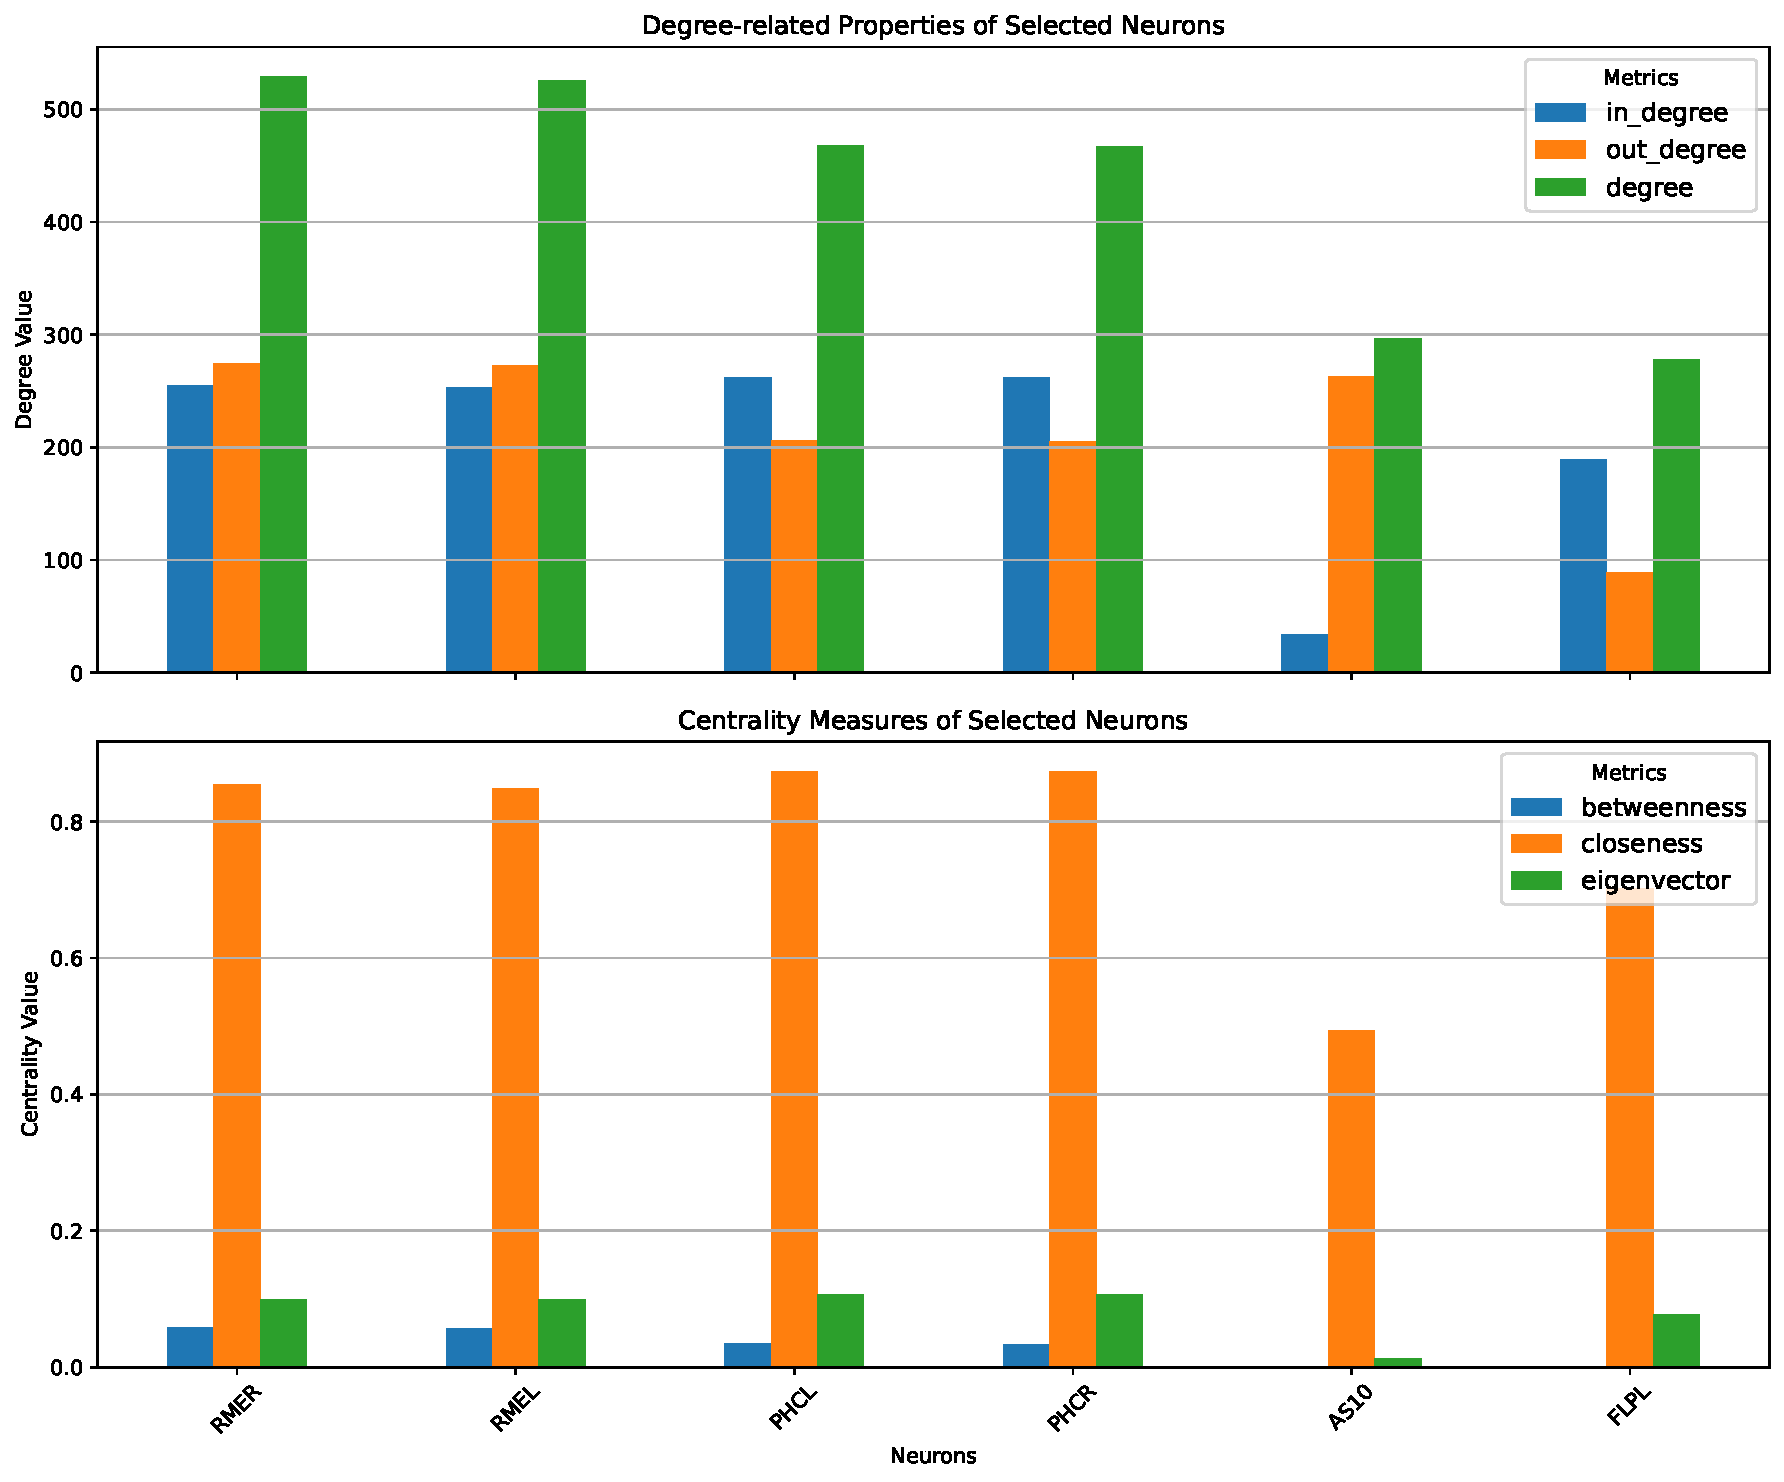
\includegraphics[width=0.6\textwidth]{./SI-figs/psg.pdf}
\caption{\textbf{Connectivity and centrality measures for the purely synaptic subgraph.}
Degree and centrality measures for the highest-degree neurons within this regime,
including RMER, RMEL, PHCL, PHCR, AS10, and FLPL. Although RMEL/RMER and PHCL/PHCR have
high total degree, most of their connections are non-significant; AS10 and FLPL
concentrate the largest number of topology-specific significant connections.}
\label{fig:SI_psg}
\end{figure*}